\section{Definition of the instances and pools of instances}

Once the multistate and multi-component types of entities used by the model have been described, using \class{SpeciesType}s and \class{Selector}s, one needs to define quantitatively actual states and connectivity of the elementary components within the \class{Species} of the SBML core. The new entity pool instances will then be used either as initial conditions or in any SBML constructs refering to \class{Species}. In order to specify these states and partnerships, we extend \class{Species} to link to \class{SpeciesTypeInstance}s, themselves refering to a list of \class{Selector}s. A \class{SpeciesTypeInstance} describes an entity that fulfils all the listed \class{Selector}s. A \class{Species} is effectively the ensemble of all the \class{SpeciesTypeInstance}s belonging to the same compartment. Note that it is the responsibility of the person or software generating the SBML file to ensure that the selectors used to precise the \class{SpeciesTypeInstance}s are not incompatible. The initial conditions, that is the intial states and connectivities of each species have to be fully specified.

\begin{figure}[h!]
\begin{center}
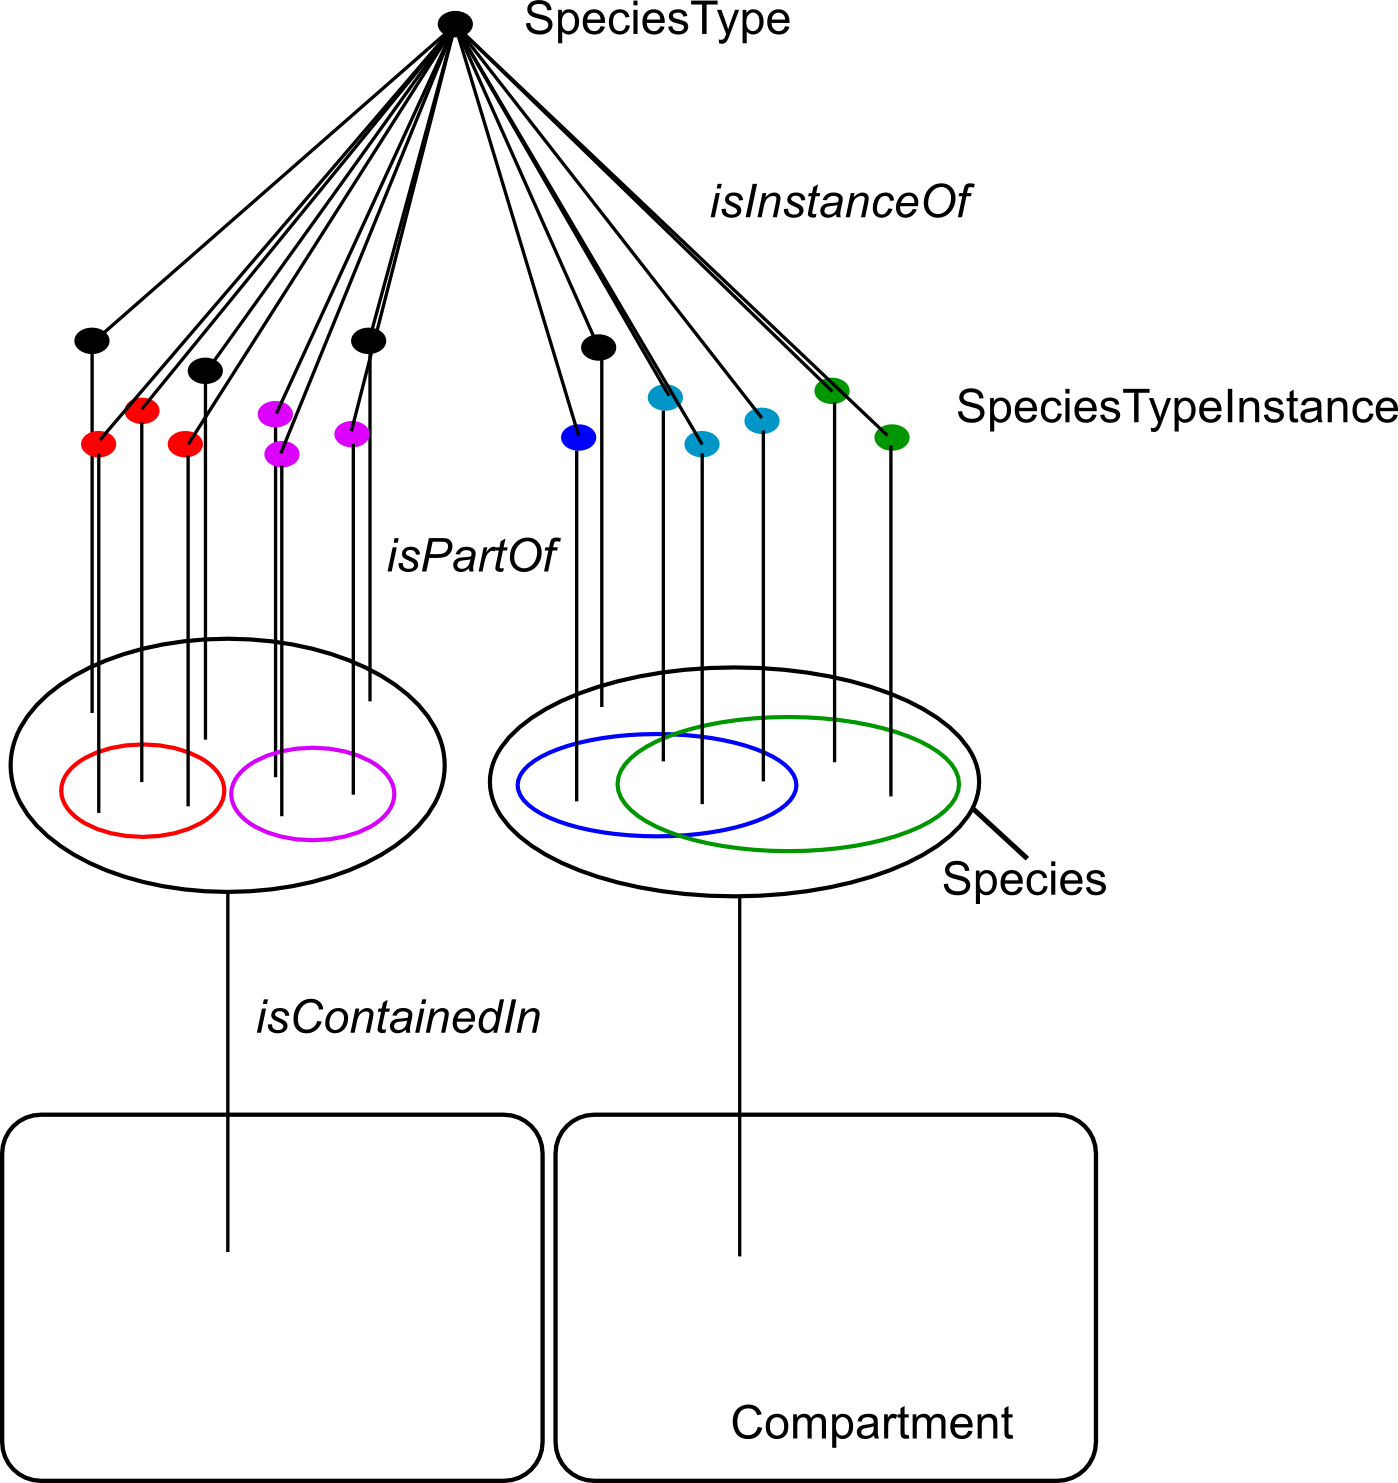
\includegraphics[scale=0.5]{./figs/pngs/Instantiation.png}
\caption{Relationships between a conceptual species type, the actual species type instances and the different pools of entities defined in a model description.}
\end{center}
\end{figure}

\begin{figure}[h!]
\begin{center}
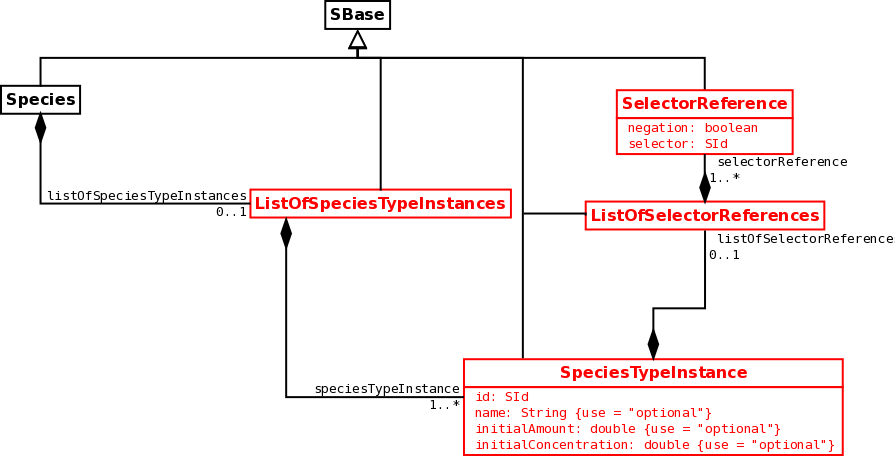
\includegraphics[scale=0.3]{./figs/pngs/SpeciesGeneral.png}
\caption{\class{Species} and all the associated classes of \multiVone.}
\end{center}
\end{figure}

Note that a ``filtered'' species is also an entity pool, and therefore is located in a given compartment. However, this species subset can be generated, selected, with a \class{Selector} that is using several SpeciesTypes instantiated by species in different compartments. Another species, located in another compartment, could be selected by a different "portion" of the same selector. This provides a mechanism to build multi-compartment entities.

\subsection{Species}

In order to encode the structures needed to refine entity pools based on their state and connectivity, we precise instances of which \class{SpeciesType} compose the \class{Species}. The element \class{Species} is then linked to a list of \class{SpeciesTypeInstance}s, each of one describing an entity part of a different pool.

\begin{figure}[H]
\begin{center}
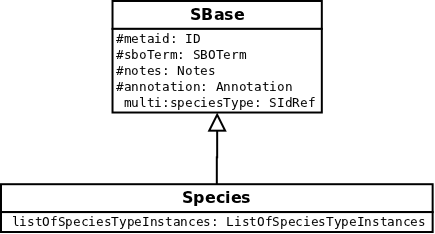
\includegraphics[scale=0.3]{figs/pngs/SpeciesClass.png} 
\caption{Definition of the extended version of \class{Species} and its relation with \class{SBase}.}
\label{fig:SpeciesClass}
\end{center}
\end{figure}

\begin{example}
<species id="species1" name="LGIC" sboTerm="SBO:0000245"
         boundaryCondition="false" hasOnlySubstanceUnit="false" constant="false"
         xmlns:multi="http://www.sbml.org/sbml/level3/version1/multi/version1"
         multi:speciesType="speciesType1" >
  <multi:listOfSpeciesTypeInstances>
    <!-- some definition of subpools -->
  </multi:listOfSpeciesTypeInstances>
</species>
\end{example}

\subsection{SpeciesTypeInstance}

A \class{SpeciesTypeInstance} is identified by an \attribute{id} and an optional \attribute{name}.  A \class{SpeciesTypeInstance} is linked to a list of \class{SelectorReference}s. When used in the SBML model, the \attribute{id} represent the either the size of the pool formed by all the \class{SpeciesTypeInstance}s that fulfil the selection, or the species type restriction. The context decides. As all elements derived from \class{SBase}, it can link to \class{Notes} and \class{Annotation}, and carry a \attribute{metaid}, and an \attribute{sboTerm}. In addition, a \class{SpeciesTypeInstance} may precise the size of the pool as an \attribute{initialAmount} or an \attribute{initialConcentration}. If neither \attribute{initialAmount} nor \attribute{initialConcentration} are precised, the instance is not to be used for initial conditions.  

\begin{figure}[H]
\begin{center}
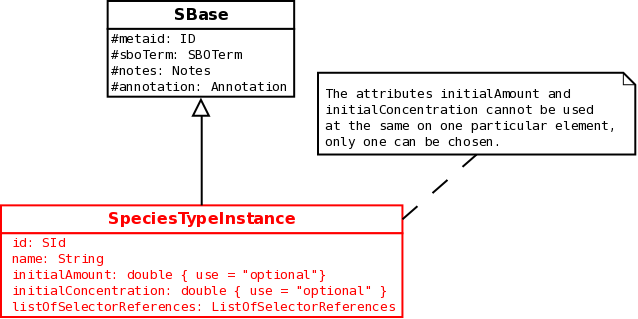
\includegraphics[scale=0.3]{figs/pngs/SpeciesTypeInstanceClass.png} 
\caption{Definition of \class{SpeciesTypeInstance} and its relation with \class{SBase}.}
\label{fig:SpeciesTypeInstanceClass}
\end{center}
\end{figure}

\begin{example}
<multi:speciesTypeInstance 
         xmlns:multi="http://www.sbml.org/sbml/level3/version1/multi/version1" 
         multi:id="SpeciesTypeInstance1"
         multi:name="LGIC_open"
         multi:initialAmount="1">
  <multi:listOfSelectorReferences>
    <!-- selectors to combine to filter out the instance -->
  </multi:listOfSelectorReferences>
</multi:speciesTypeInstance>
\end{example}

Note that because an instance can fulfill several selectors, the selectors used to create instances used as initial conditions may overlap. As a consequence, the sum of all the initial quantities may be larger than the initial quantity specified on the \class{Species}. It is up to the modeler generating the description to make sure there is no ambiguity and that whatever procedure is used to create the instances result in the same distribution.

\class{SpeciesTypeInstance}s defined in a \class{Species} inherit the value of the attribute \attribute{hasOnlySubstanceUnit} carried by the \class{Species}. In other words, regardless of the presence of the attributes \attribute{initialAmount} and \attribute{initialConcentration} carried by a \class{SpeciesTypeInstance}, when used in a context requiring a quantity its \attribute{id} represents an amount if  the \class{species}' \attribute{hasOnlySubstanceUnit} is set to \cdata{true}. 

\subsection{SelectorReference}\label{sec:SelectorReference}

As all elements derived from \class{SBase}, A \class{SelectorReference}  can link to \class{Notes} and \class{Annotation}, and carry a \attribute{metaid}, and an \attribute{sboTerm}. It targets a \class{Selector} through its \attribute{selector} attribute. A boolean attribute \attribute{negation} allows to precise that the entities fulfilling the rules described in the selector are NOT selected.

\begin{figure}[H]
\begin{center}
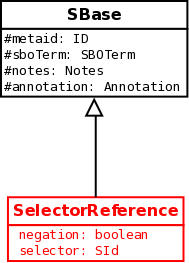
\includegraphics[scale=0.3]{figs/pngs/SelectorReferenceClass.png} 
\caption{Definition of \class{SelectorReference} and its relation with \class{SBase}.}
\label{fig:SelectorReferenceClass}
\end{center}
\end{figure}

\begin{example}
<multi:selectorReference 
         xmlns:multi="http://www.sbml.org/sbml/level3/version1/multi/version1" 
         multi:selector="selector1"
         multi:negation="true" />
\end{example}

\subsection{Complete description of a species with pools of instances}\label{exampleSpecies}

The example below describes the encoding of two instances of the speciesType \cdata{speciesType1}. 

\begin{example}
<species id="species1" 
         boundaryCondition=false" hasOnlySubstanceUnit=false" constant=false"
         compartment="compartment1" initialAmount="1000"
         xmlns:multi="http://www.sbml.org/sbml/level3/version1/multi/version1"
         multi:speciesType="speciesType1" >
  <multi:listOfSpeciesTypeInstances>
    <multi:SpeciesTypeInstance multi:id="speciesTypeInstance1" 
                               multi:initialAmount="1">
      <multi:listOfSelectorReferences>
        <multi:selectorReference multi:selector="selector1" multi:negation="false"/>
      <multi:listOfSelectorReferences>
    </multi:speciesTypeInstance>
    <multi:speciesTypeInstance multi:id="speciesTypeInstance2">
      <multi:listOfSelectorReferences>
        <multi:selectorReference multi:selector="selector2" multi:negation="false"/>
        <multi:selectorReference multi:selector="selector3" multi:negation="true" />
      <multi:listOfSelectorReferences>
    </multi:speciesTypeInstance>
  </multi:listOfSpeciesTypeInstances>
</species>
\end{example}

\begin{figure}[H]
\begin{center}
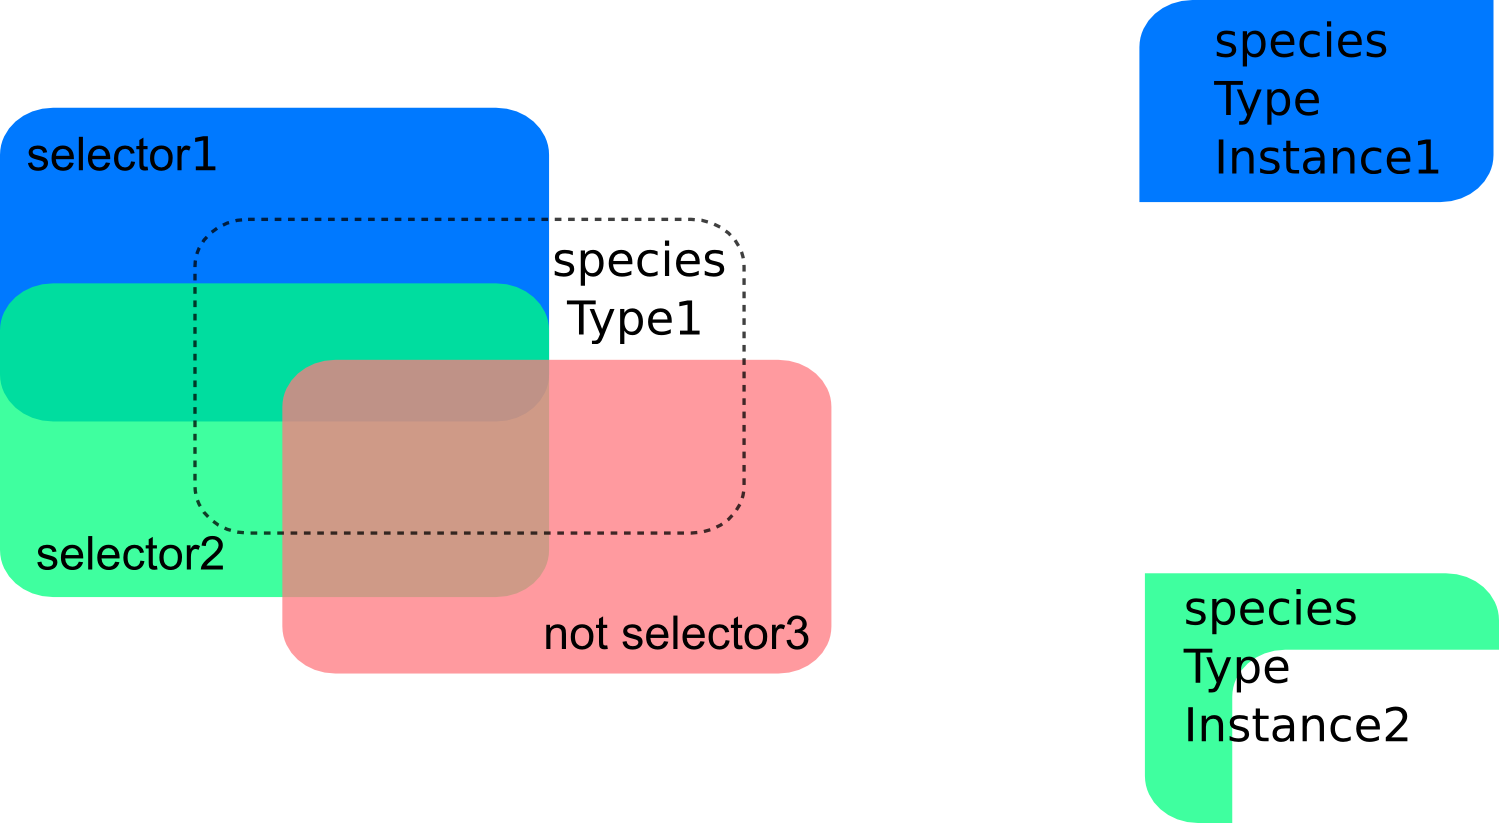
\includegraphics[scale=0.4]{figs/pngs/speciesTypeInstanceBuilding.png}
\caption{Procedure to build speciesTypeInstances from a speciesType and selectors. The dashed rectangle represent all the instances of a species, in all possible states and connectivity. Selector1 is used to generate the entity pool SpeciesTypeInstance1. Selector2 and Selector3 are used in combination to generate SpeciesTypeInstance2.}
\label{fig:speciesTypeInstanceBuilding}
\end{center}
\end{figure}


